% Stage 2: Ontology-Guided Extraction - Process and Results Comparison
% Alternative figure showing extraction flow and result comparison

\begin{figure*}[t]
\centering

% Top part: Process Flow
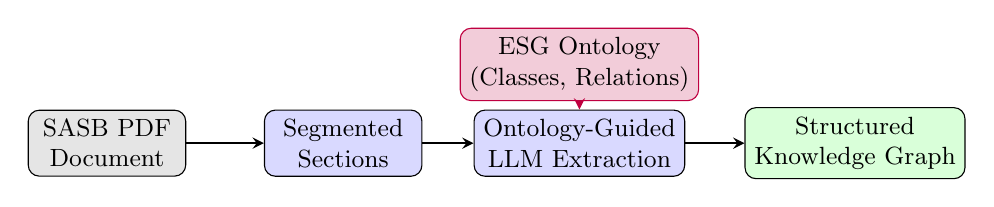
\begin{tikzpicture}[
    node distance=0.6cm,
    box/.style={rectangle, draw, rounded corners, minimum width=2cm, minimum height=0.6cm, align=center, font=\small},
    input/.style={box, fill=gray!20},
    ontology/.style={box, fill=purple!20, draw=purple},
    process/.style={box, fill=blue!15},
    output/.style={box, fill=green!15},
    arrow/.style={->, >=stealth, thick},
]

% Process Flow
\node[input] (doc) at (0, 0) {SASB PDF\\Document};
\node[process] (seg) at (3, 0) {Segmented\\Sections};
\node[ontology] (ont) at (6, 1) {ESG Ontology\\(Classes, Relations)};
\node[process] (ext) at (6, 0) {Ontology-Guided\\LLM Extraction};
\node[output] (kg) at (9.5, 0) {Structured\\Knowledge Graph};

\draw[arrow] (doc) -- (seg);
\draw[arrow] (seg) -- (ext);
\draw[arrow, purple] (ont) -- (ext);
\draw[arrow] (ext) -- (kg);

\end{tikzpicture}

\vspace{0.8cm}

% Bottom part: Results Comparison Table
\renewcommand{\arraystretch}{1.2}
\begin{tabular}{p{3.5cm}|p{5.5cm}|p{5.5cm}}
\toprule
\textbf{Aspect} & \textbf{Baseline Extraction} & \textbf{Ontology-Guided Extraction} \\
\midrule
\textbf{Entity Recognition} &
\textcolor{red!70!black}{``GHG emissions'', ``carbon output'', ``Scope 1''} (inconsistent naming) &
\textcolor{green!50!black}{\texttt{esg:GrossGlobalScope1Emissions}} (standardised URI) \\
\midrule
\textbf{Relationships} &
\textcolor{red!70!black}{None extracted; entities are isolated} &
\textcolor{green!50!black}{\texttt{Metric} $\xrightarrow{isCalculatedBy}$ \texttt{Model}} \\
\midrule
\textbf{Calculation Logic} &
\textcolor{red!70!black}{Embedded in free text; not machine-readable} &
\textcolor{green!50!black}{\texttt{hasFormula: ``(scope1 + scope2) / revenue''}} \\
\midrule
\textbf{Data Provenance} &
\textcolor{red!70!black}{No link to data sources} &
\textcolor{green!50!black}{\texttt{Metric} $\xrightarrow{obtainedFrom}$ \texttt{CO2DIRECTSCOPE1}} \\
\midrule
\textbf{Confidence Scoring} &
\textcolor{red!70!black}{Not available} &
\textcolor{green!50!black}{\texttt{hasConfidenceScore: 100}} \\
\midrule
\textbf{Output Format} &
\textcolor{red!70!black}{Unstructured JSON/text} &
\textcolor{green!50!black}{RDF triples (613 triples extracted)} \\
\bottomrule
\end{tabular}

\caption{Stage 2: Ontology-guided extraction process and results comparison. The top panel shows the extraction pipeline where the ESG ontology schema constrains LLM extraction to produce semantically consistent outputs. The bottom table compares extraction results: baseline approaches produce fragmented, inconsistent entities without relationships, while ontology-guided extraction yields standardised entities with explicit semantic relationships, calculation formulas, and confidence-scored data provenance links.}
\label{fig:stage2_extraction}
\end{figure*}
